\documentclass[tikz,border=3pt]{standalone}
\usepackage{pgfplots}
\usepgfplotslibrary{groupplots}
\pgfplotsset{compat=1.18}
\begin{document}
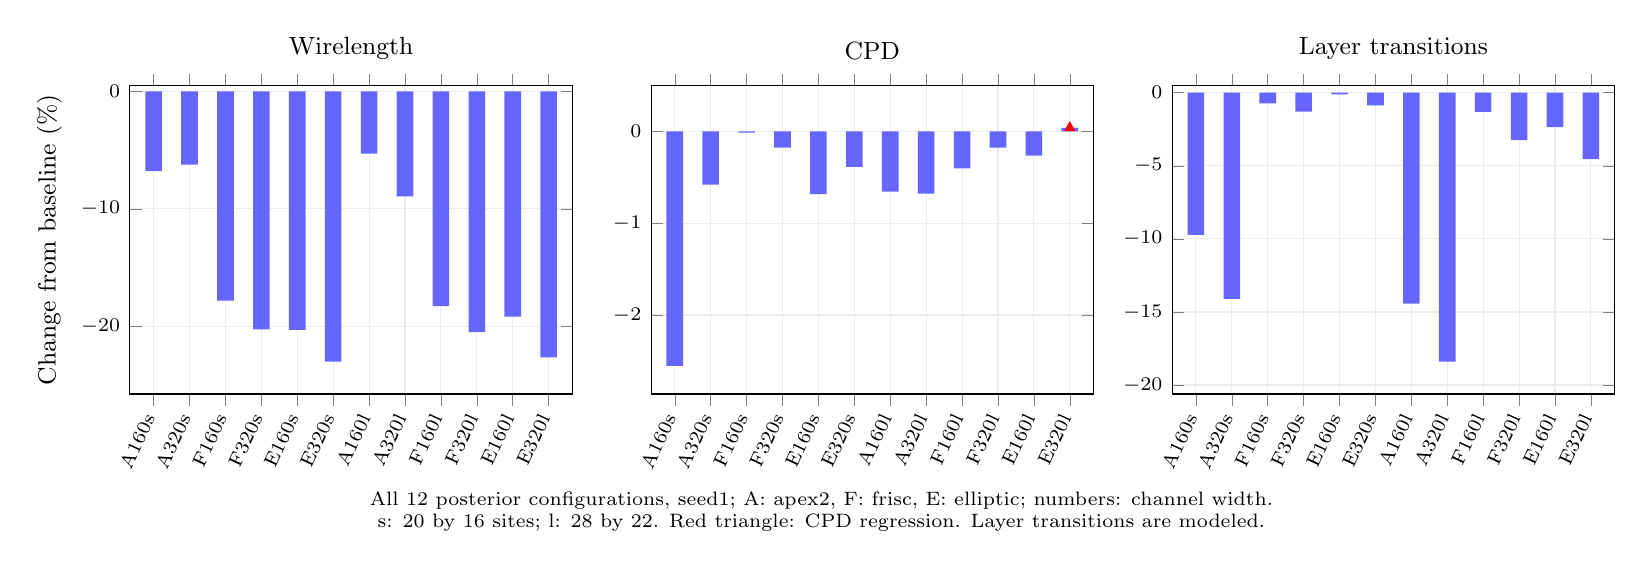
\begin{tikzpicture}
\begin{groupplot}[group style={group size=3 by 1,horizontal sep=1cm},width=7.2cm,height=5.5cm,ybar,/pgf/bar width=6pt,xtick={1,2,3,4,5,6,7,8,9,10,11,12},xticklabels={A160s,A320s,F160s,F320s,E160s,E320s,A160l,A320l,F160l,F320l,E160l,E320l},xticklabel style={rotate=65,anchor=east},enlarge x limits=.06,grid=major,grid style={gray!15},tick label style={font=\scriptsize},label style={font=\small},title style={font=\small}]
\nextgroupplot[title={Wirelength},ylabel={Change from baseline (\%)},ymin=-25.75120612997824,ymax=.5]
\addplot[fill=blue!60,draw=none] coordinates {(1,-6.789020626928699) (2,-6.245568101238208) (3,-17.808311443389236) (4,-20.263648284905788) (5,-20.302025262860766) (6,-22.992148330337713) (7,-5.303030303030298) (8,-8.939409525768948) (9,-18.27631191347894) (10,-20.48302278776861) (11,-19.1754030882587) (12,-22.645555758350067)};
\nextgroupplot[title={CPD},ymin=-2.859033752481802,ymax=.5]
\addplot[fill=blue!60,draw=none] coordinates {(1,-2.552708707573037) (2,-0.5798741248850825) (3,-0.012826679493349591) (4,-0.17650267963159605) (5,-0.6843879284591292) (6,-0.3881858244026981) (7,-0.655179135977213) (8,-0.6773906031153243) (9,-0.40361209265802334) (10,-0.17855176428021036) (11,-0.263100197325139) (12,0.03838587399835891)};
\addplot[only marks,mark=triangle*,red,mark size=2pt] coordinates {(12,0.03838587399835891)};
\nextgroupplot[title={Layer transitions},ymin=-20.60949208992507,ymax=.5]
\addplot[fill=blue!60,draw=none] coordinates {(1,-9.733777038269553) (2,-14.097598760650653) (3,-0.7311586051743535) (4,-1.2965050732807182) (5,-0.10632642211589882) (6,-0.857908847184985) (7,-14.42141623488774) (8,-18.40133222314738) (9,-1.3144590495449915) (10,-3.2435129740518986) (11,-2.355350742447515) (12,-4.53857791225416)};
\end{groupplot}
\node[anchor=north,font=\scriptsize,align=center] at (current bounding box.south) {All 12 posterior configurations, seed1; A: apex2, F: frisc, E: elliptic; numbers: channel width.\\s: 20 by 16 sites; l: 28 by 22. Red triangle: CPD regression. Layer transitions are modeled.};
\end{tikzpicture}
\end{document}
